\section{Подготовка окружения}

\subsection{Ход работы}

\subsubsection{Подготовка окружения для виртуализации}


В данной работе используется программа \textit{VMPlayer} для виртуализации и
образ виртуальной машины, предоставляемый компанией \textit{SearchInform} в
учебных целях. Конфигурация тривиальна и не использует дополнительных настроек,
в качестве хоста используется операционная система на базе ядра
\textit{linux 4.11}.

\subsubsection{Смена пароля}

Для смены пароля необходимо зайти в панель управления компьютером $\rightarrow$
администрирование $\rightarrow$ управление компьютером $\rightarrow$ служебные
программы $\rightarrow$ пользователи $\rightarrow$ Администратор.

\begin{figure}[H]
  \centering
  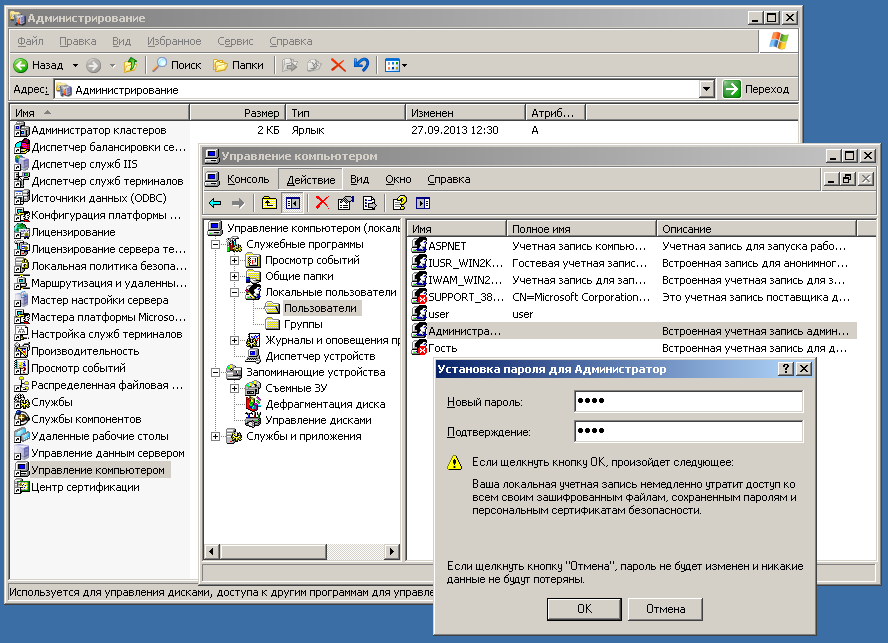
\includegraphics[width=\textwidth]{passwd}
  \caption{Изменение пароля администратора.}\label{fig:passwd}
\end{figure}

\subsubsection{Изменение пароля доступа к консолям основных серверов}

Изменить пароли можно с помощью программ \textit{Search Server Console},
\textit{SearchInform DataCenter}, \textit{SearchInform EndpointSniffer},
\textit{SearchInform NetworkSniffer}, \textit{SearchInform ReportCenter
Console}, \textit{SearchInform AlertCenter Client} как показано на
рис.~\ref{fig:passwdSrv}~-~\ref{fig:passwdRC}.

\begin{figure}[H]
  \centering
  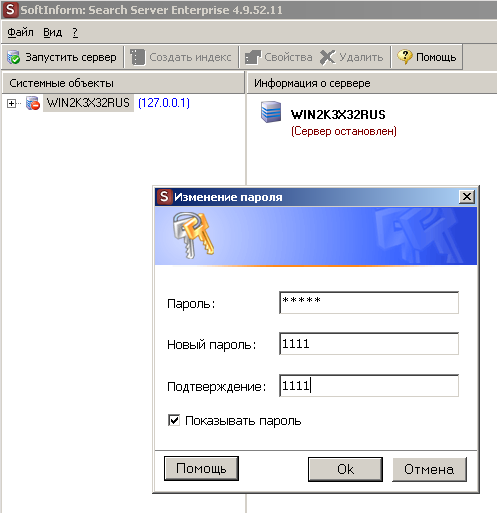
\includegraphics[width=0.7\textwidth]{passwdSrv}
  \caption{Изменение пароля сервера.}\label{fig:passwdSrv}
\end{figure}

\begin{figure}[H]
  \centering
  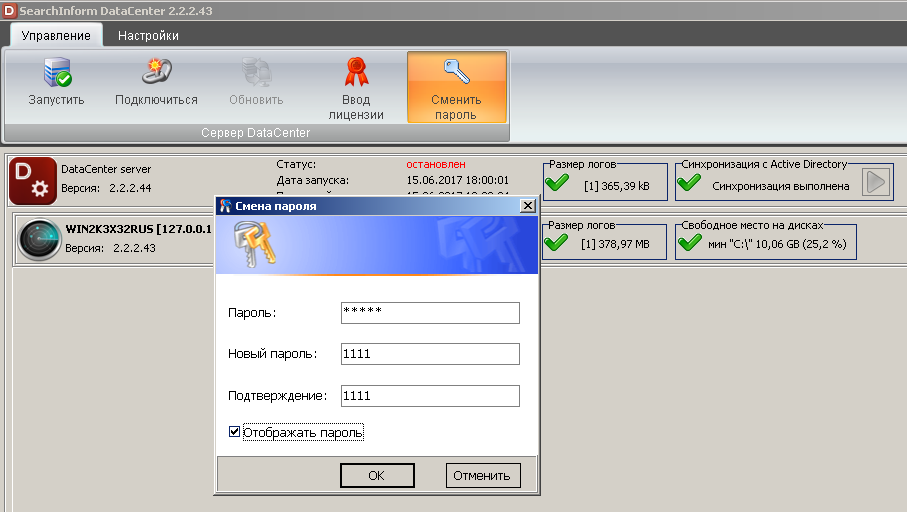
\includegraphics[width=0.7\textwidth]{passwdDC}
  \caption{Изменение пароля DataCenter.}\label{fig:passwdDC}
\end{figure}

\begin{figure}[H]
  \centering
  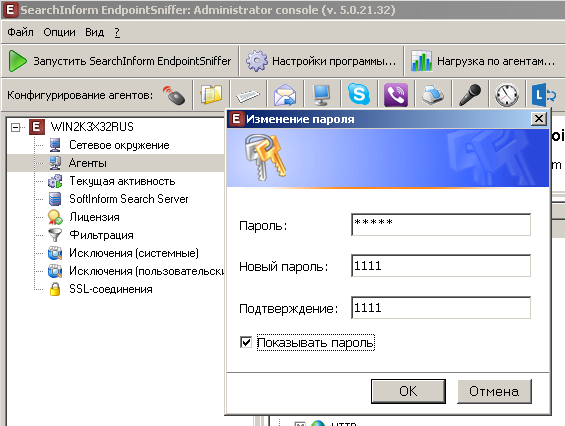
\includegraphics[width=0.7\textwidth]{passwdES}
  \caption{Изменение пароля EndpointSniffer.}\label{fig:passwdES}
\end{figure}

\begin{figure}[H]
  \centering
  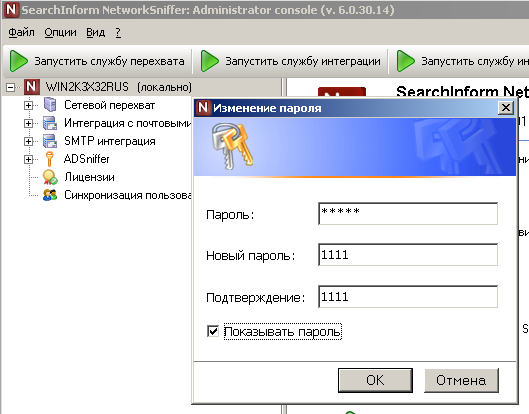
\includegraphics[width=0.7\textwidth]{passwdNS}
  \caption{Изменение пароля NetworkSniffer.}\label{fig:passwdNS}
\end{figure}

\begin{figure}[H]
  \centering
  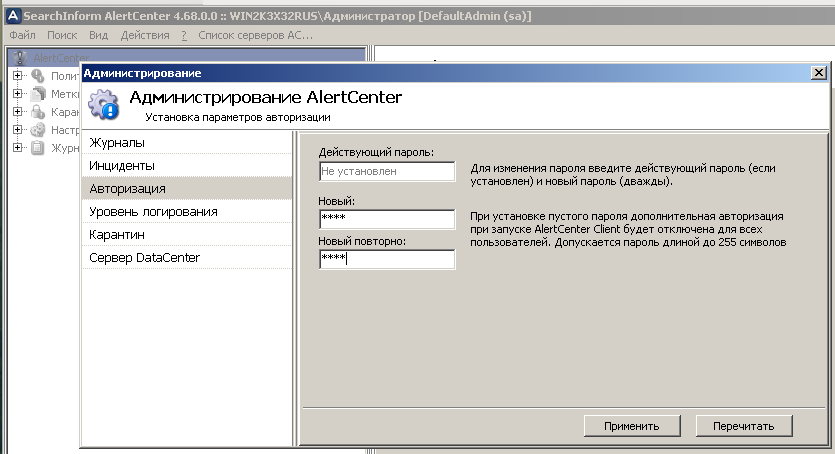
\includegraphics[width=0.7\textwidth]{passwdAC}
  \caption{Изменение пароля AlertCenter.}\label{fig:passwdAC}
\end{figure}

\begin{figure}[H]
  \centering
  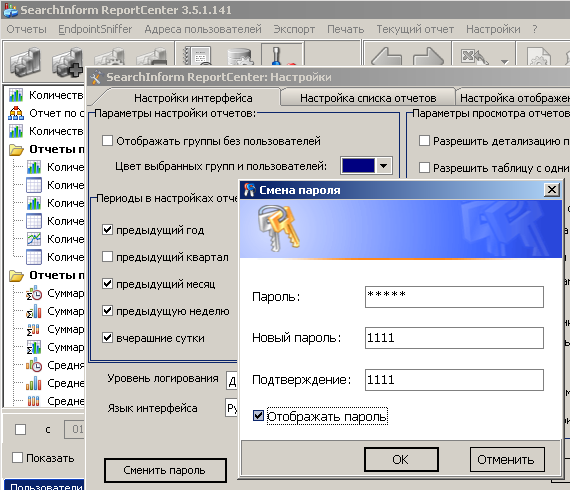
\includegraphics[width=0.7\textwidth]{passwdRC}
  \caption{Изменение пароля ReprotCenter.}\label{fig:passwdRC}
\end{figure}

\subsubsection{Ограничить права доступа пользователей к индексам Search Server}

Это можно сделать с помощью \textit{SearchIorm Server Console}, см. рис.~
\ref{fig:fpRight}.

\begin{figure}[H]
  \centering
  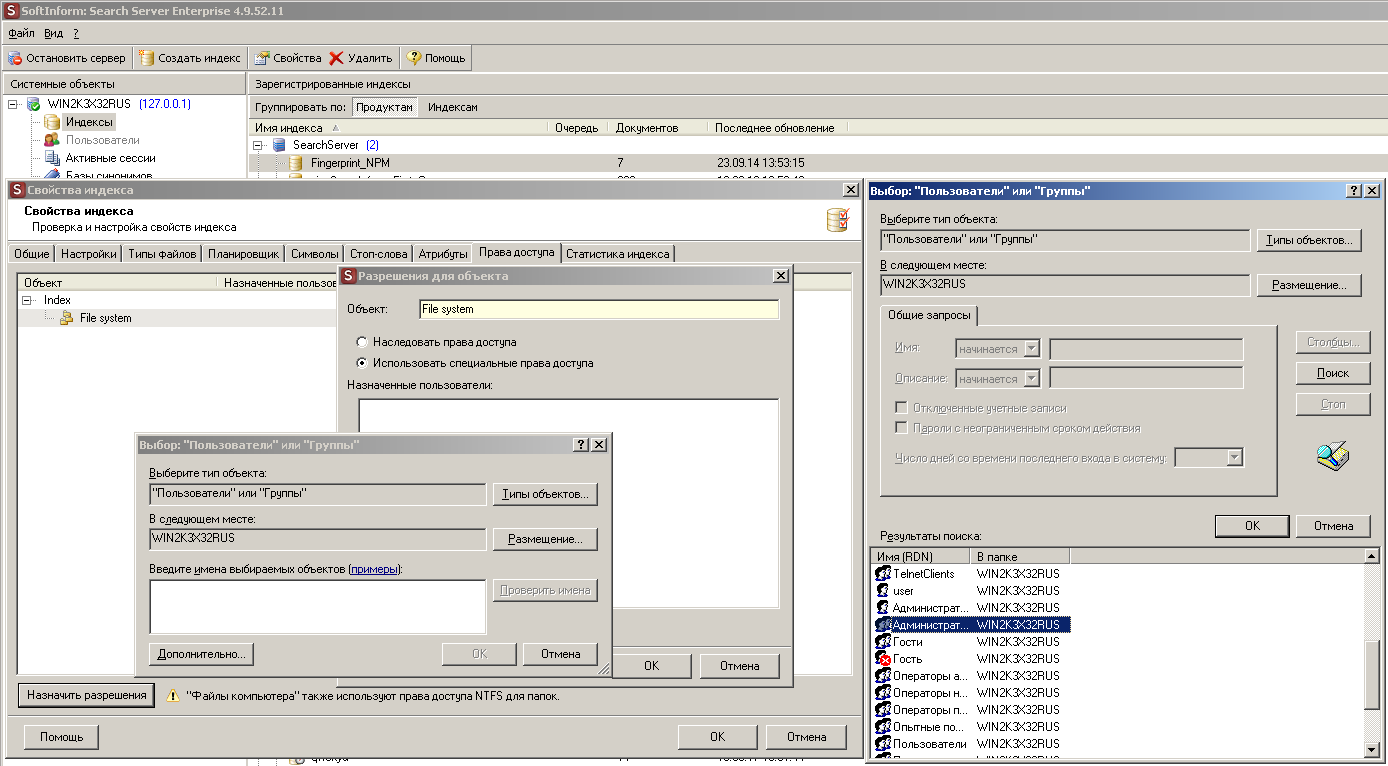
\includegraphics[width=\textwidth]{fingerprintRight.png}
  \caption{Изменение пароля ReprotCenter.}\label{fig:fpRight}
\end{figure}

\subsubsection{Управление пользователями системных служб SearchInform}

Установим в качестве пользователя, от имени которого работает сервас
\textit{SearchInform AlertCenter server} Администартора, рис.
\ref{fig:serviceAdmin}.

\begin{figure}[H]
  \centering
  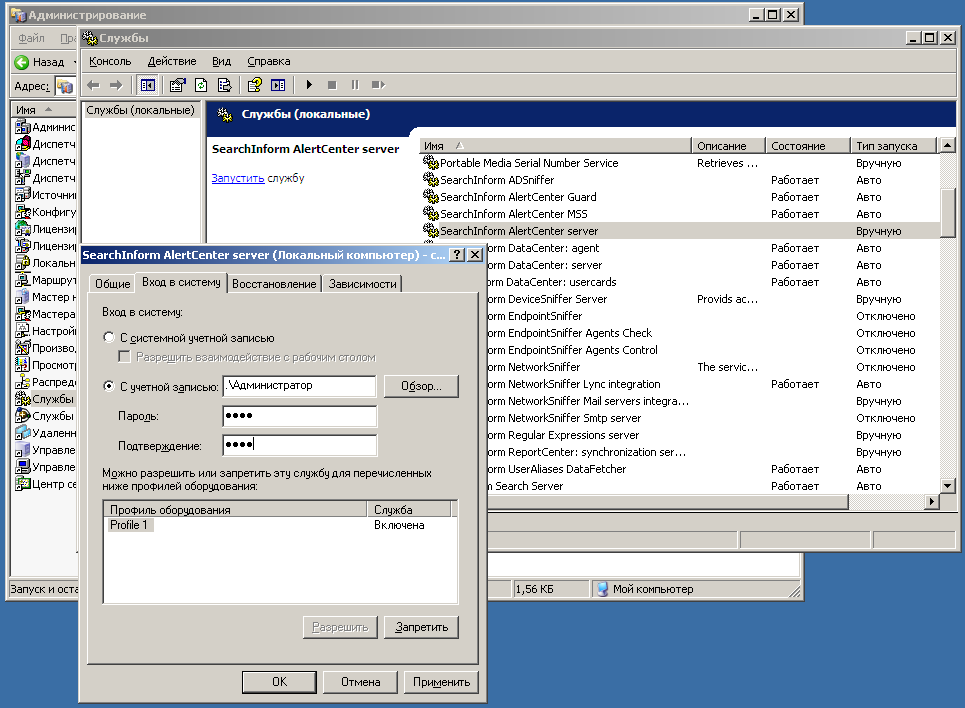
\includegraphics[width=\textwidth]{serviceAdmin}
  \caption{Установка администратора в качестве пользователя для
  AlertCenter server.}\label{fig:serviceAdmin}
\end{figure}

\subsubsection{Настройка параметров функционирования SearchInform AlertCenter}

Настроим \textit{AlertCenter}, как на рис. \ref{fig:acConfig}.

\begin{figure}[H]
  \centering
  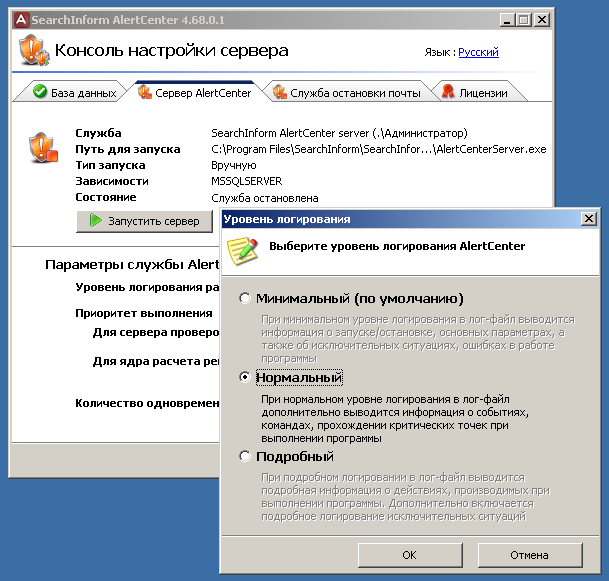
\includegraphics[width=\textwidth]{acConfig}
  \caption{Настройка AlertCenter.}\label{fig:acConfig}
\end{figure}

\subsubsection{Настройка системной службы SearchInform DataCenter : agent}

Настроим автоматический запуск этой службы, как на рис. \ref{fig:dcaAutorun}.

\begin{figure}[H]
  \centering
  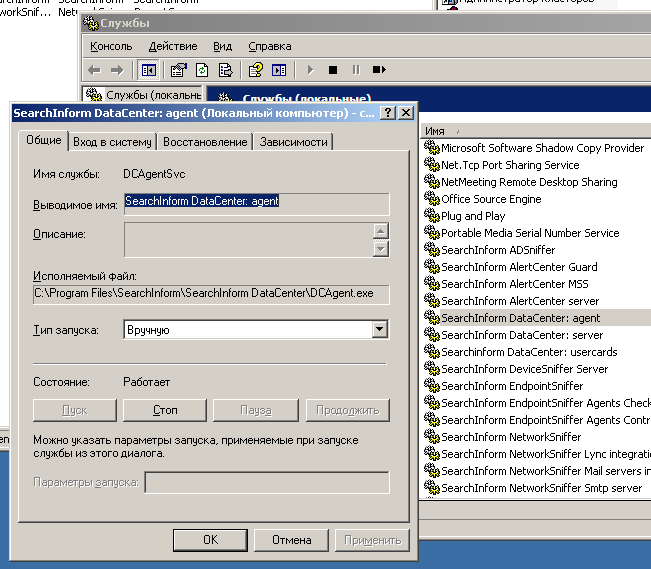
\includegraphics[width=\textwidth]{dcaAutorun}
  \caption{Настройка Автозапуска DataCenter: agent.}\label{fig:dcaAutorun}
\end{figure}

\subsubsection{Настройка параметров функционирования SearchInform
EndpointSniffer}

Аналогично настроим автозапуск \textit{EndpointSniffer}, см рис.
\res{esAutorun}.

\begin{figure}[H]
  \centering
  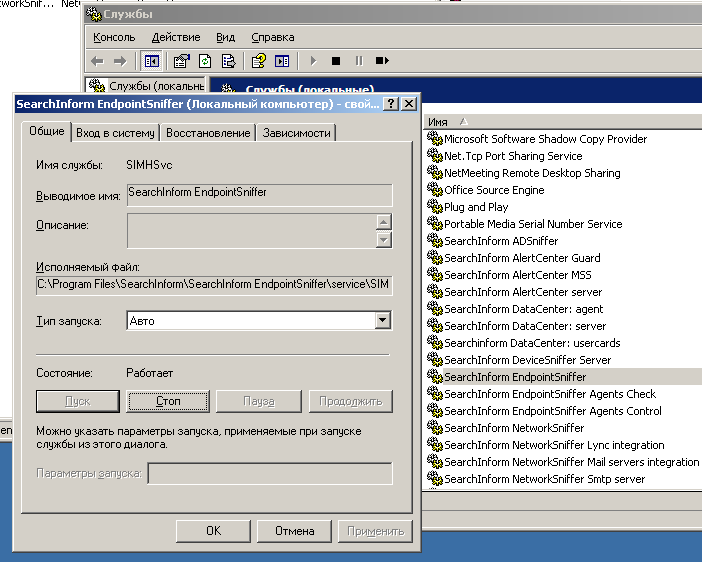
\includegraphics[width=\textwidth]{esAutorun}
  \caption{Настройка Автозапуска EndpointSniffer.}\label{fig:esAutorun}
\end{figure}

\subsection{Контрольные вопросы}

\begin{itemize}
  \item Для чего необходим перехват всех документов, покидающих периметр
    организации, независимо от каналов, по которым это делается?

    Для контроля пользователей, обладающей информацией, содержащейся в
    документах. Для контроля местонахождения документов (в случае физических
    носителей).

  \item Требуется ли системный администратор в штате службы информационной
    безопасности и почему?

    Требуется для оперативной настройки специфических средств для обеспечения
    информационной безопасности. Также для оперативного добавления и
    \администрирования прав доступа пользователей.

  \item По каким схемам можно включить контур информационной безопасности в
    сеть предприятия?
  \item Какая из схем подключения наиболее оптимальна при наличии технической
    возможности?
  \item Перечислите основные аппаратные требования для штатного
    функционирования операционной системы Windows Server 2003?

    Процессор с тактовой частотой 400 МГц;
    минимум 512 МБ ОЗУ;
    для сетевой установки: 1,2 ГБ;
    для установки с компакт-диска: 2,9 ГБ;

  \item Что такое индекс?

    Ассоциативный массив значения какой-либо функции от данных, на
    соответствующие данные.
 \end{itemize}
